\documentclass[10pt,landscape]{scrartcl}
\usepackage{multicol}
\usepackage{calc}
\usepackage{ifthen}
\usepackage[landscape]{geometry}
% Umlaute ermöglichen
\usepackage[T1]{fontenc}
% Format dieses Dokuments
\usepackage[utf8]{inputenc}
% Deutsche Trennungsregeln
\usepackage[ngerman]{babel}
\usepackage[babel,german=quotes]{csquotes}
\usepackage{wrapfig}
\usepackage{listings}
\lstloadlanguages{ada}
\lstset{emph={%  
    wiederhole, bis, solange, setze, gebe%
    },emphstyle={\bfseries}%
}
%%\usepackage{color}
%\definecolor{lightgrey}{gray}{0.75}
%\definecolor{darkgrey}{gray}{0.25}

\usepackage{amssymb,amsmath,amsthm}
\newtheorem*{satz}{Satz}

\usepackage{tikz}
\usetikzlibrary{arrows,automata,chains,shapes.arrows}

\usepackage{ulem}

\usepackage{hyperref}
%\pdfoutput=1
\hypersetup{
	pdfauthor   = {Lazari, Constantin},
	pdftitle    = {Informatik Cheat Sheet},
	pdfsubject  = {Informatik},
	pdfkeywords = {},
	pdfcreator  = {Kile},		% Texnic Center oder Kile z.B.
	pdfproducer = {pdflatex},
	colorlinks  = false		% Links nicht farbig hervorheben (sieht Scheisse aus).
} 

% To make this come out properly in landscape mode, do one of the following
% 1.
%  pdflatex latexsheet.tex
%
% 2.
%  latex latexsheet.tex
%  dvips -P pdf  -t landscape latexsheet.dvi
%  ps2pdf latexsheet.ps

% This sets page margins to .5 inch if using letter paper, and to 1cm
% if using A4 paper. (This probably isn't strictly necessary.)
% If using another size paper, use default 1cm margins.
\ifthenelse{\lengthtest { \paperwidth = 11in}}
	{ \geometry{top=.5in,left=.5in,right=.5in,bottom=.5in} }
	{\ifthenelse{ \lengthtest{ \paperwidth = 297mm}}
		{\geometry{top=1cm,left=1cm,right=1cm,bottom=1cm} }
		{\geometry{top=1cm,left=1cm,right=1cm,bottom=1cm} }
	}

% Turn off header and footer
\pagestyle{empty}
 
% Redefine section commands to use less space
\makeatletter
\renewcommand{\section}{\@startsection{section}{1}{0mm}%
                                {-1ex plus -.5ex minus -.2ex}%
                                {0.5ex plus .2ex}%x
                                {\normalfont\large\bfseries}}
\renewcommand{\subsection}{\@startsection{subsection}{2}{0mm}%
                                {-1explus -.5ex minus -.2ex}%
                                {0.5ex plus .2ex}%
                                {\normalfont\normalsize\bfseries}}
\renewcommand{\subsubsection}{\@startsection{subsubsection}{3}{0mm}%
                                {-1ex plus -.5ex minus -.2ex}%
                                {1ex plus .2ex}%
                                {\normalfont\small\bfseries}}
\newcommand{\msout}[1]{\text{\sout{\ensuremath{#1}}}}
\makeatother

% Define BibTeX command
\def\BibTeX{{\rm B\kern-.05em{\sc i\kern-.025em b}\kern-.08em
    T\kern-.1667em\lower.7ex\hbox{E}\kern-.125emX}}

% Don't print section numbers
\setcounter{secnumdepth}{0}
\setlength{\parindent}{0pt}

\setlength{\parskip}{0pt plus 0.5ex}


% -----------------------------------------------------------------------

\begin{document}

	\raggedright
	\footnotesize
	\begin{multicols}{3}


	% multicol parameters
	% These lengths are set only within the two main columns
	%\setlength{\columnseprule}{0.25pt}
	\setlength{\premulticols}{1pt}
	\setlength{\postmulticols}{1pt}
	\setlength{\multicolsep}{1pt}
	\setlength{\columnsep}{2pt}
	\newlength{\MyLenA}
	\newlength{\MyLenB}

	\begin{center}
	\Large{\textbf{Informatik Cheat Sheet}} \\
	\end{center}

	\section{Rechnerarchitektur}
\subsection{Von-Neumann-Rechner}
Kennzeichen:
\begin{itemize}\itemsep0em
	\item Der Rechner ist universell oder Turing mächtig	
	\item Programm und Daten liegen im gleichen beschreibbaren Speicher auf den beliebig zugegriffen werden kann (RAM -- Random Access Memory). Zwischen Programm und Programmdaten wird nicht unterschieden. Hier ist auch das grösste Risiko. Programm oder Daten können beabsichtigt oder unbeabsichtigt beschädigt werden
	\item Programm und Daten sind binär codiert
	\item Steuerung erfolgt über Befehle in einem Programm
	\item Ohne korrektes Programm ist der Rechner nutzlos
	\item Programm = Sequenz von Anweisungen/Entscheidungen
	\item Der Befehlszähler (spez. Speicher) kennt Adresse des nächsten Befehls
	\item Bedingte Befehle erlauben Entscheidungen über den Fortgang des Programms
\end{itemize}

\subsubsection{Komponenten}
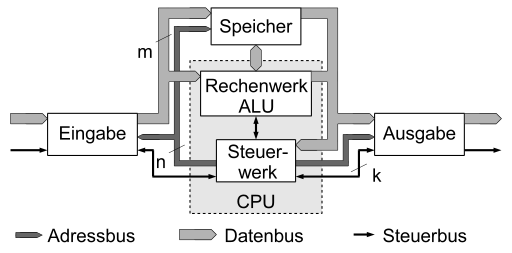
\includegraphics[width=\linewidth]{von_Neumann-_Architektur_de.png}
\begin{description}\itemsep0em
	\item [Steuerwerk] (Leitwerk/\textit{Control Unit}) enthält Befehlsregister, Befehlsdecoder und den Befehlszähler:
	\begin{itemize}
		\item Interpretiert Programmcode
		\item Erstellt Verbindungen zwischen Speicher und Rechenwerk
		\item Steuert die Reihenfolge der Programmbefehle
	\end{itemize}

	\item [Rechenwerk] (Arithmetisch-Logische-Einheit, \textit{Arithmetic Logic Unit (ALU)}) stellt logische und mathematische Operationen (NICHT, ODER, \dots, Addition, Multiplikation, \dots) zur Verfügung

	Steuer- und Rechenwerk zusammen bilden heutzutage zusammen (mit weiteren Komponenten) die \textit{Central Processing Unit (CPU)} (aka. Hauptprozessor)

	\item [Speicher(werk)] (\textit{Memory}) Speichert alle Daten (alles im selben Speicher). Der Speicher ist in fortlaufend durchnummerierte gleich grosse Zellen unterteilt. Die Nummer entspricht der Adresse der Speicherzelle
	\item [Eingabewerk] Steuert die Eingabe aller Daten des Rechners 
	\item [Ausgabewerk] Steuert die Ausgabe aller Daten des Rechners

	Ein- und Ausgabewerk zusammen sind letztendlich dedizierte Speicher. Sie sind heutzutage in der \textit{Input/Output-Unit (I/O-Unit)} zusammengefasst
\end{description}

Die einzelnen Werke sind über Bus-Systeme (Daten-, Adress- und Steuerbus) miteinander verknüpft.

\subsubsection{Register}
Register (Teil des Steuer- und Rechenwerks) sind sehr schnelle, sehr kleine Speicher für die Zwischenspeicherung von Daten. Steuer- und Rechenwerk arbeiten i.\,d.\,R. mit Werten dieser Register

\begin{itemize}\itemsep0em
	\item Befehlsregister (im Steuerwerk)
	\item Befehlszähler (im Steuerwerk)
	\item Zustandsregister (im Steuerwerk)
	\item Interrupt-Register (im Steuerwerk)
	\item Akkumulator (im Rechenwerk)
	\item Statusregister (im Rechenwerk)
	\item Hilfs- und Arbeitsregister (\textit{General Purpuse Register}, Steuer- und Rechenwerk)
\end{itemize}

Die Grösse der Register (i.\,d.\,R. $n \cdot 8$) charakterisiert einen Rechner:
\begin{itemize}\itemsep0em
	\item Akkumulator/Arbeitsregister definiert Grösse der in einem Zyklus bearbeitbaren Zahlen
	(Bei 32 Bit $\rightarrow 2^{32}$ mögliche Zahlen)
	\item Befehlszähler definiert die Grösse des direkt ansprechbaren Speichers
	\item Befehlsregister definiert die Anzahl möglicher Befehle
\end{itemize}
Für Register gilt: je grösser, desto teuerer. Üblich sind 8, 16, 32 und 64 Bit Register

Ein Register besteht aus $n$ Flip-Flops, die einzeln angesprochen werden können

\subsubsection{Programmablauf}
\begin{enumerate}\itemsep0em
	\item Aktuelles Befehlswort aus der Speicherzelle, auf die der Befehlszähler zeigt lesen und and das Steuerwerk übertragen
	\item Befehlswort dekodieren und entsprechende Signale auf die Steuerleitungen schalten
	\item Operanden aus dem Speicherwerk lesen und in die Register des Rechenwerks übertragen
	\item Operation ausführen und Ergebnis in ein Register oder den Speicher schreiben
	\item Befehlszähler um eins erhöhen (oder aufgrund eines Sprungbefehls auf einen anderen Wert setzen)
\end{enumerate}

\subsubsection{Von-Neumann-Flaschenhals}
Die Trennung von Recheneinheit und Speicher führt dazu, dasss Daten sehr häufig übertragen werden müssen. Somit wird der Zuständige Datenbus zum Flaschenhals (Von-Neumann-Flaschenhals).
Auf dem Datenbus werden sowohl Programmcode als auch Daten übertragen und das ganze geschieht sequentiell.

Lösungsansätze:
\begin{itemize}\itemsep0em
	\item Schneller Zwischenspeicher zwischen CPU und Speicher (Cache)
	\item Getrennte Busse und Zwischenspeicher für Programmcode und Daten
	\item Vorhersagen von bedingten Programmverzweigungen (\textit{branch prediction})
	\item Parallele Strukturen
\end{itemize}

\subsection{Harvard-Architektur}
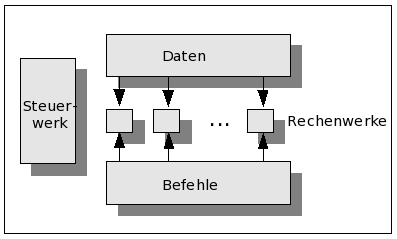
\includegraphics[width=\linewidth]{Harvard-architektur.png}
\begin{itemize}\itemsep0em
	\item Trennt Programm- und Datenspeicher (inkl. Zwischenspeicher)
	\item Nutzt getrennte Datenbusse
	\item kann mehrere Rechenwerke parallel nutzen
\end{itemize}

 \begin{tabular}{@{}p{\linewidth/2}%
				@{}p{\linewidth/2}}
	\multicolumn{1}{c}{\underline{Linksverschiebung}} & \multicolumn{1}{c}{\underline{Rechtsverschiebung}}\\
	Programm und Daten werden gleichzeitig geladen & Nichtdeterministisches Verhalten aufgrund unterschiedlicher Laufzeiten \\
	Programmcode kann nicht überschrieben werden & Nicht genutzer Speicherplatz der einen Art kann nicht für die andere genutzt werden \\
	Befehlswortbreite und Datenwortbreite können unterschiedlich sein & \\

\end{tabular}

\subsubsection{Super-Harvard-Architektur}
Auf gemeinsamen Speicher wird über verschiedene Datenbusse parallel zugegriffen


	% !TEX root = Informatik-3.tex
\section{Prozessor}
Eigenschaften:
\begin{description}\itemsep0em
	\item [Befehlssatz] Die Befehle, die hardwareseitig implementiert sind. Je grösser deren Anzahl, desto kürzere und damit schnellere Programme sind möglich. Ein Compiler macht aus einem Programmbefehl $n$ Prozessorbefehle (Befehlsarchitektur)
	\item [Taktzyklus] beschreibt die Dauer eines Zykluses (normalerweise in Hz also Taktzyklen pro Sekunde angegeben)
	\item [Taktzyklen pro Befehl (CPI)] (\textit{clock cyles per instruction}) gibt an, wieviele Taktzyklen ein Befehl im Durchschnitt benötigt (Einzelne Befehle gehen schneller 1 Taktzyklus, andere langsamer $>$ 1 Taktzyklus)
\end{description}

\subsection{Befehl laden}
Befehlszähler addressiert Speicherzelle, der Inhalt wird ins Befehlsregister übertragen
(für arithmetisch-logische Operationen). Dazu sind Schaltnetze und Schaltwerke erforderlich.
\begin{description}\itemsep0em
	\item [Schaltnetz] besteht ausschliesslich aus logischen Bauelementen (AND, ADD, \dots)
	\begin{itemize}\itemsep0em
		\item besteht aus $2^n$ Dateneingängen, $n$ Steuereingängen und einem Ausgang. 	Mit Hilfe der Steuereingänge wird bestimmt, welches der $n$-Eingangssignale durchgeleitet wird
		\item Kombinationen von Schaltnetzen sind wieder ein Schaltnetz
	\end{itemize}

	\item [Schaltwerk] speichert intern Daten
	\begin{itemize}\itemsep0em
		\item mindestens ein Dateneingang, ein Datenausgang und ein Takteingang
		\item Takteingang bestimmt, wann ein Speicherelement überschrieben wird (gelesen werden kann es immer)
		\item Unterscheidung zwischen pegel- und flankengesteuerten Schaltwerken (heute: Flanken), d.\,h. die Spannung muss einen bestimmten Wert übersteigen, damit Schreibvorgänge stattfinden
	\end{itemize}	
\end{description}

Allgemein: Schaltwerk $\rightarrow$ Schaltnetz $\rightarrow$ Schaltwerk
Bei flankengesteuerten Schaltwerken können die Daten wieder ins selbe Schaltwerk geschrieben werden


\subsection{Befehl}
Besteht aus Operationscode (OP-Code), ggf. Optionen und Operanden.

z.B. OP-Code, (Option), Operand-1, Operand-2, (Operand-3) 
\subsection{Operanden laden, speichern}
Mit Hilfe von Schaltnetzen und -werken werden Daten aufgrund der von der ALU berechneten  absolute Speicheradresse manipuliert

\subsection{Ablaufzeit eines Programms $P$}
\begin{equation*}
	t_P = \mbox{(Anzahl Befehle)} \cdot \mbox{CPI} \cdot \mbox{Zeit pro Zyklus}
\end{equation*}

Die minimale Zykluszeit hängt davon ab, wie lange der Strom entlang des längsten möglichen Datenpfades für einen Befehl braucht. Optimierung muss sich immer nach diesem Befehl richten,
auch wenn der Befehl nur selten gebraucht wird. Alle anderen Befehle müssen immer auf den langsamsten aller möglichen Befehle warten.

Load/Store unter Einbezug des Speichers ist wohl immer am langsamsten.

Befehle können gruppiert werden, so dass alle Befehle einer Gruppe etwa gleich lange Pfade haben. Langsamere Befehle beanspruchen dann einfach $n$ Zyklen (so kommt dann der CPI-Wert zustande). Allerdings wird dann die Steuerung und das Design deutlich komplexer.

\subsection{Pipelining}
Mehrere Befehle werden gleichzeitig (überlappend ausgeführt).

\subsubsection{Konflikte}
\begin{description}
\item[Strukturkonflikte] gleichzeitiger Zugriff auf Ressourcen. --> gelöst durch Pipeline-Architektur und abgestimmten Befehlssatz
\item[Datenkonflikte] Abwarten von Zwischenresultaten --> Compiler, Forwarding
\item[Steuerkonflikte] z.b. bedingte Sprünge --> Branch-Prediction
\end{description}

\subsubsection{Zykluszeit}
Die Zykluszeit ist vorgegeben durch die Stufe mit der grössten Zeit, ein Befehl benötigt daher mehr Zeit (bei gleichbleibender Taktrate).

Ein Programm wird bei n-stufiger Pipeline n mal schneller abgearbeitet als bei einem Prozessor ohne Pipeline, falls die längste Stufe gleiche Taktzykluszeit benötigt wie ein Zyklus des Prozessors ohne Pipeline.







	
	\rule{0.3\linewidth}{0.25pt}\\
	\scriptsize
	Copyright \copyright\ 2013 Constantin Lazari\\
	% Should change this to be date of file, not current date.
	Revision: 1.0, Datum: \today\\
	\end{multicols}
\end{document}